%DIF 1c1
%DIF LATEXDIFF DIFFERENCE FILE
%DIF DEL /dev/fd/63             Wed Jan  6 15:54:39 2016
%DIF ADD ./latex-diff-org.tex   Wed Jan  6 15:54:39 2016
%DIF < % Created 2016-01-06 Wed 15:35
%DIF -------
% Created 2016-01-06 Wed 15:54 %DIF > 
%DIF -------
\documentclass[11pt]{article}
\usepackage[utf8]{inputenc}
\usepackage{lmodern}
\usepackage[T1]{fontenc}
\usepackage{fixltx2e}
\usepackage{graphicx}
\usepackage{longtable}
\usepackage{float}
\usepackage{wrapfig}
\usepackage{rotating}
\usepackage[normalem]{ulem}
\usepackage{amsmath}
\usepackage{textcomp}
\usepackage{marvosym}
\usepackage{wasysym}
\usepackage{amssymb}
\usepackage{amsmath}
\usepackage[version=3]{mhchem}
\usepackage[numbers,super,sort&compress]{natbib}
\usepackage{natmove}
\usepackage{url}
\usepackage{minted}
\usepackage{underscore}
\usepackage[linktocpage,pdfstartview=FitH,colorlinks,
linkcolor=blue,anchorcolor=blue,
citecolor=blue,filecolor=blue,menucolor=blue,urlcolor=blue]{hyperref}
\usepackage{attachfile}
\author{John Kitchin}
\date{\today}
\title{latex-diff-org}
%DIF PREAMBLE EXTENSION ADDED BY LATEXDIFF
%DIF UNDERLINE PREAMBLE %DIF PREAMBLE
\RequirePackage[normalem]{ulem} %DIF PREAMBLE
\RequirePackage{color}\definecolor{RED}{rgb}{1,0,0}\definecolor{BLUE}{rgb}{0,0,1} %DIF PREAMBLE
\providecommand{\DIFadd}[1]{{\protect\color{blue}\uwave{#1}}} %DIF PREAMBLE
\providecommand{\DIFdel}[1]{{\protect\color{red}\sout{#1}}}                      %DIF PREAMBLE
%DIF SAFE PREAMBLE %DIF PREAMBLE
\providecommand{\DIFaddbegin}{} %DIF PREAMBLE
\providecommand{\DIFaddend}{} %DIF PREAMBLE
\providecommand{\DIFdelbegin}{} %DIF PREAMBLE
\providecommand{\DIFdelend}{} %DIF PREAMBLE
%DIF FLOATSAFE PREAMBLE %DIF PREAMBLE
\providecommand{\DIFaddFL}[1]{\DIFadd{#1}} %DIF PREAMBLE
\providecommand{\DIFdelFL}[1]{\DIFdel{#1}} %DIF PREAMBLE
\providecommand{\DIFaddbeginFL}{} %DIF PREAMBLE
\providecommand{\DIFaddendFL}{} %DIF PREAMBLE
\providecommand{\DIFdelbeginFL}{} %DIF PREAMBLE
\providecommand{\DIFdelendFL}{} %DIF PREAMBLE
%DIF END PREAMBLE EXTENSION ADDED BY LATEXDIFF

\begin{document}

\tableofcontents

\section{Word-based diffs for org-mode}
\label{sec-1}

When we write manuscripts we often want or need to see how one version differs from another. latexdiff is pretty good for this, and today we consider how to use it when your org-file is in git. It turns out we can use git to retrieve the old versions for comparison.

\begin{minted}[frame=lines,fontsize=\scriptsize,linenos]{sh}
git hist
\end{minted}

\begin{verbatim}
* 4ff3b06 Wed Jan 6 13:32:32 2016 | initial commit (HEAD -> master) [John Kitchin]
\end{verbatim}

You can see above, at the time I ran the command there was one commit. As we develop the manuscript, we periodically export the result to see how it looks. At some point, all the changes should be committed \emph{including the tex file}. We will use the different versions of the org and tex files to generate latexdiffs.

\subsection{Generating diffs}
\label{sec-1-1}
Supposing you have a commit that represents some interesting point in the past, e.g. a submitted version, or the last edits made by a collaborator, here is how we generate a diff of the changes between the current version and that version.

First, check out your history. We will compare the current version to the commit \texttt{6f9a77a}.

\begin{minted}[frame=lines,fontsize=\scriptsize,linenos]{sh}
git hist
\end{minted}

\begin{verbatim}
* 6f9a77a Wed Jan 6 13:37:03 2016 | successful build. we will compare to this version later. (HEAD -> master) [John Kitchin]
* 26fdf5c Wed Jan 6 13:34:20 2016 | new files added, tex and pdf [John Kitchin]
* 4ff3b06 Wed Jan 6 13:32:32 2016 | initial commit [John Kitchin]
\end{verbatim}

\begin{minted}[frame=lines,fontsize=\scriptsize,linenos]{sh}
git diff --color-words  --word-diff=plain 6f9a77a -- latex-diff-org.org
\end{minted}

\subsection{Generating the latexdiff}
\label{sec-1-2}

Run this in a bash shell (it doesn't work for me in org-mode I suppose because it is using sh, not bash). I find latexdiff somewhat on the fragile side, for example you cannot make changes in section headings or the latexdiff result won't compile. So we ignore those commands below. Somewhat unfortunate, but livable I suppose.

\begin{minted}[frame=lines,fontsize=\scriptsize,linenos]{sh}
latexdiff --exclude-textcmd="section,subsection" <(git show 6f9a77a:latex-diff-org.tex) latex-diff-org.tex > diff.tex
\end{minted}

It works like this, however.
\begin{minted}[frame=lines,fontsize=\scriptsize,linenos]{common-lisp}
(shell-command "latexdiff --exclude-textcmd=\"section,subsection\" <(git show 6f9a77a:latex-diff-org.tex) latex-diff-org.tex > diff.tex")
\end{minted}

\begin{verbatim}
0
\end{verbatim}

Now compile the diff to get the pdf:

\begin{minted}[frame=lines,fontsize=\scriptsize,linenos]{sh}
pdflatex -shell-escape diff.tex
pdflatex -shell-escape diff.tex
\end{minted}


\DIFdelbegin \DIFdel{Here is the diff: }%DIFDELCMD < 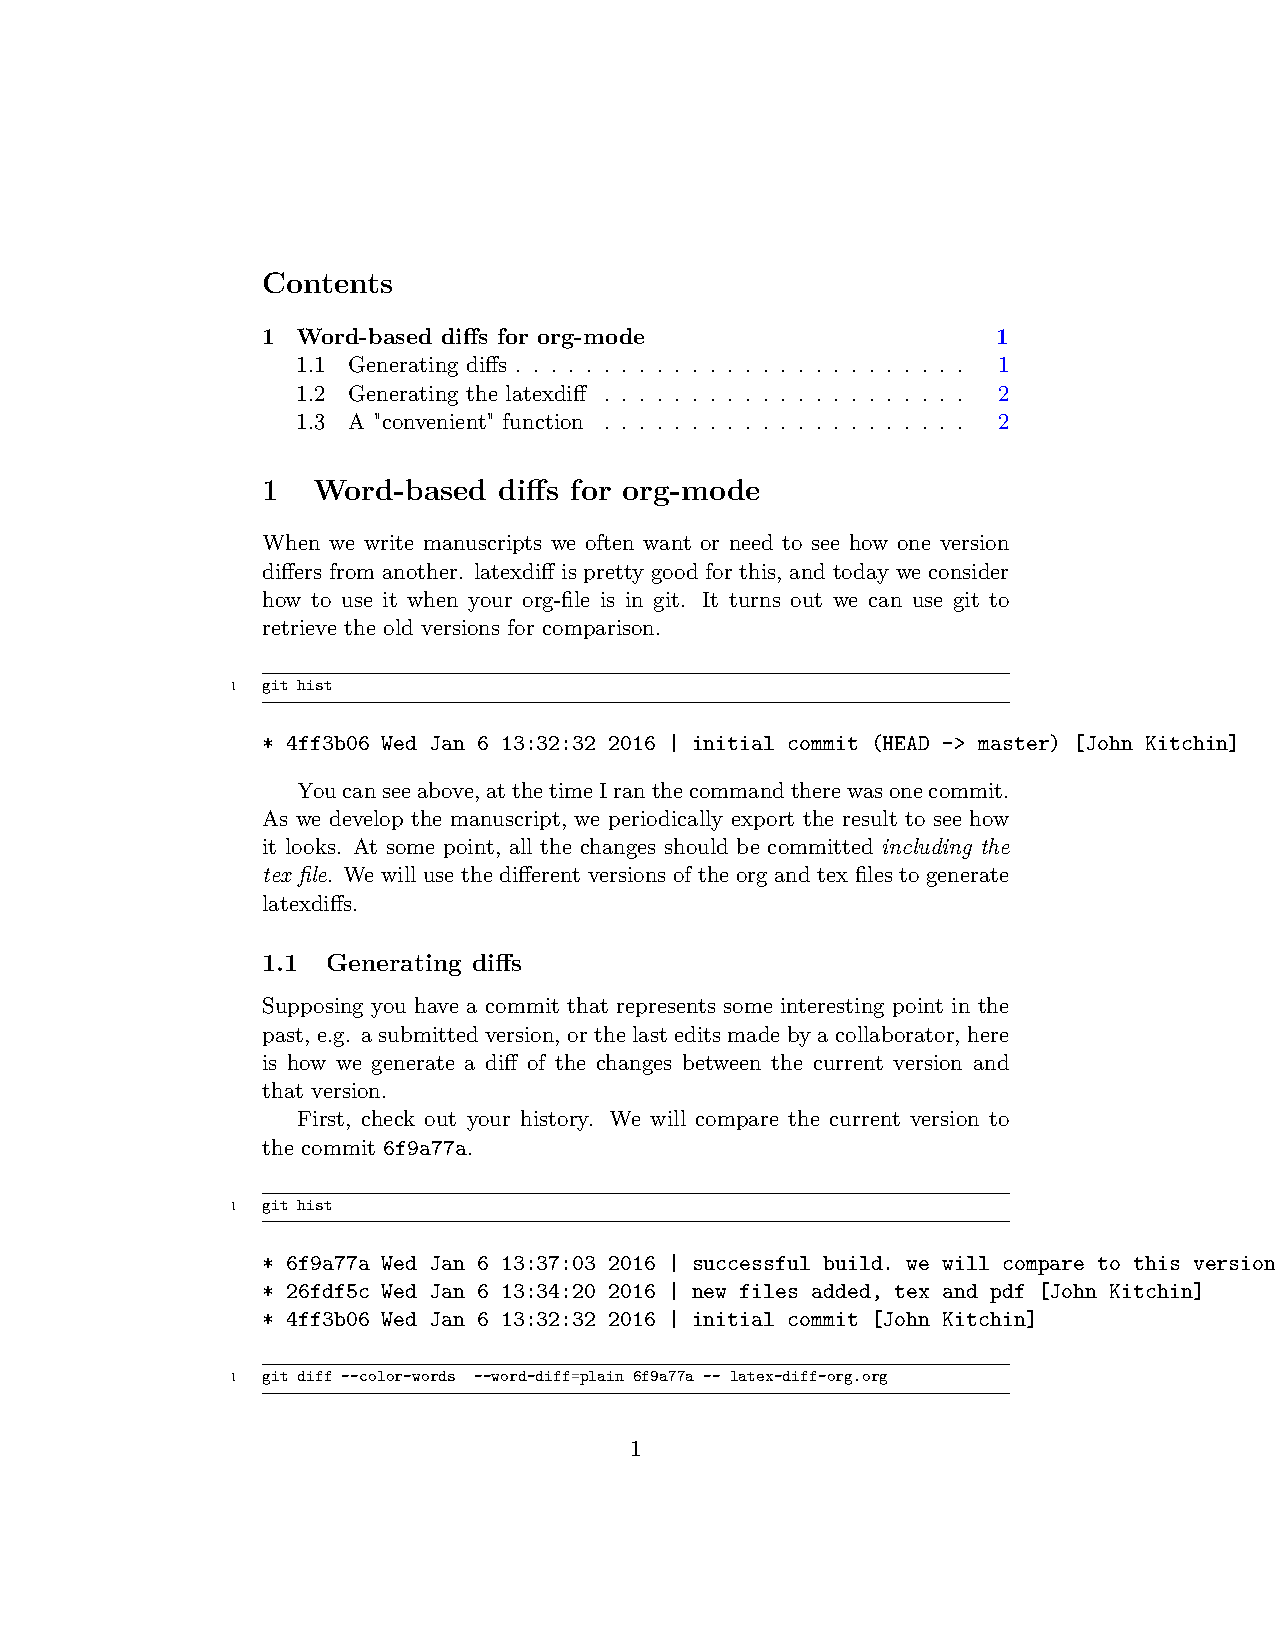
\includegraphics[width=.9\linewidth]{diff.pdf}
%DIFDELCMD < 

%DIFDELCMD < %%%
\DIFdelend \DIFaddbegin \subsection{A "convenient" function}
\label{sec-1-3}
\DIFaddend So, we might as well get ourselves a convenient function for that. Helm is my goto selector, so here we grab some candidates based on the commits.

\begin{minted}[frame=lines,fontsize=\scriptsize,linenos]{common-lisp}
(mapcar (lambda (s)
          (let ((commit (nth 1 (split-string s)))
                msg)
          (string-match "|.*\DIFdelbegin \DIFdel{$" s)
          (cons (concat commit " " (match-string 0 s)) commit)))
        (split-string (shell-command-to-string "git hist") "\n"))
\end{minted}

\begin{minted}[frame=lines,fontsize=\scriptsize,linenos]{common-lisp}
(("6f9a77a | successful build. we will compare to this version later. (HEAD -> master) [John Kitchin]" . "6f9a77a")
 ("26fdf5c | new files added, tex and pdf [John Kitchin]" . "26fdf5c")
 ("4ff3b06 | initial commit [John Kitchin]" . "4ff3b06"))
\end{minted}


\begin{minted}[frame=lines,fontsize=\scriptsize,linenos]{common-lisp}
(defun latexdiff (commit)
  (let ((fname (concat (file-name-base (buffer-file-name)) ".tex")))
    (shell-command (format
                    "latexdiff --exclude-textcmd=\"section,subsection\" <(git show %s:%s) %s > diff.tex"
                    commit fname fname))
    (shell-command "pdflatex -shell-escape diff.tex")
    (shell-command "pdflatex -shell-escape diff.tex")
    (org-open-file "diff.pdf")))

(helm :sources `((name . "commits")
                 (candidates . ,(mapcar (lambda (s)
                                         (let ((commit (nth 1 (split-string s)))
                                               msg)
                                           (string-match "|.*$}\DIFdelend \DIFaddbegin \DIFadd{$" s)
          (cons (concat commit " " (match-string 0 s)) commit)))
        (split-string (shell-command-to-string "git hist") "\n"))
\end{minted}

\begin{minted}[frame=lines,fontsize=\scriptsize,linenos]{common-lisp}
(("6f9a77a | successful build. we will compare to this version later. (HEAD -> master) [John Kitchin]" . "6f9a77a")
 ("26fdf5c | new files added, tex and pdf [John Kitchin]" . "26fdf5c")
 ("4ff3b06 | initial commit [John Kitchin]" . "4ff3b06"))
\end{minted}

Here is the new function that calls helm to select a commit, and then runs our latexdiff function.

\begin{minted}[frame=lines,fontsize=\scriptsize,linenos]{common-lisp}
(defun latexdiff (commit)
  "Export to LaTeX and do a latexdiff from the version in COMMIT."
  (save-buffer)
  (let* ((fname (org-latex-export-to-latex))
         (cmd (format
               "latexdiff --exclude-textcmd=\"section,subsection\" <(git show %s:%s) %s > diff.tex"
               commit fname fname)))
    (message cmd)

    (shell-command cmd)
    (shell-command "pdflatex -shell-escape -interaction nonstopmode diff.tex")
    (shell-command "pdflatex -shell-escape -interaction nonstopmode diff.tex")
    (org-open-file "diff.pdf")))

(helm :sources `((name . "commits")
                 (candidates . ,(mapcar (lambda (s)
                                         (let ((commit (nth 1 (split-string s)))
                                               msg)
                                           (string-match "|.*$}\DIFaddend " s)
                                           (cons (concat commit " " (match-string 0 s)) commit)))
                                       (split-string (shell-command-to-string "git hist") "\n")))
                 (action . (lambda (commit)
                             (latexdiff commit)))))
\end{minted}

\DIFdelbegin %DIFDELCMD < \begin{minted}[frame=lines,fontsize=\scriptsize,linenos]{sh}
%DIFDELCMD < %%%
\DIFdel{git hist
}%DIFDELCMD < \end{minted}
%DIFDELCMD < 

%DIFDELCMD < \begin{verbatim}%DIFDELCMD < 
%DIFDELCMD < * 6f9a77a Wed Jan 6 13:37:03 2016 | successful build. we will compare to this version later. (HEAD -> master) [John Kitchin]
%DIFDELCMD < * 26fdf5c Wed Jan 6 13:34:20 2016 | new files added, tex and pdf [John Kitchin]
%DIFDELCMD < * 4ff3b06 Wed Jan 6 13:32:32 2016 | initial commit [John Kitchin]
%DIFDELCMD < \end{verbatim}
%DIFDELCMD < %%%
\DIFdelend \DIFaddbegin \DIFadd{It works, but it is probably limited to tex files in the root git directory.
}\DIFaddend % Emacs 25.0.50.1 (Org mode 8.2.10)
\end{document}